\documentclass{paper}

\usepackage{tikz}

\title{De Gennes's gas kinetic theory of slip}
\author{Nat Lund}

\begin{document}

\maketitle
We seek to replicate the work of de Gennes. In his elegant little paper of 2002 in Langmuir, entitled simply ``On Fluid/Wall Slippage", he presented a gas kinetic expression for slip length.  However, the paper seems to contain a few typographical errors, and the result is stated in terms of the non-standard quantity $\bar{v}_{z}$, which is apparently defined as the average of the \emph{absolute value} of the $z$ component of velocity.

As an exercise, we derive the expression from scratch using the more standard scalar quantity of particle \emph{speed}, $v$, with our final expression in terms of $\bar{v}$.  Our results ultimately agree with those of de Gennes --- we show that $\bar{v} = 4 \bar{v}_{z}$.

\vspace{1em}
We start by figuring out the number of gas molecules hitting a surface per second, then calculate the momentum transferred to get a shear stress, from which a slip length follows.

\subsubsection*{Particle Rain Rate Density}

Consider a gas of density $\rho$.  If the mass of each particle is $m$, then the \emph{number} density of the gas is $\rho / m$.

Each particle in the gas has a different velocity. The directions of motion will be uniformly distributed over all solid angles. In an ideal gas, the speeds come from the Maxwell-Boltzmann distribution.  In general, each gas particle has speed $v$ with some probability $P(v)$.

\vspace*{1em}
Our strategy is to split the gas into separate ensembles of particles, each ensemble defined as a group of particles \textbf{all with the same speed} $v_{ens}$.
At the end of the derivation, we will sum over all ensembles --- for now we work with a single arbitrary ensemble, identified by its speed $v_{ens}$.

\vspace{1em}
Consider a layer of gas over some area $A$ on the surface. Let the layer width be $l$, where $l$ is well under the \emph{mean free path} in the gas. So, particles within the layer are sparsely distributed, and we can assume they do not interact.

The ensemble indexed by $v_{ens}$ contributes
\[ \frac{\rho}{m} A l P(v_{ens}) \]
atoms to the layer.

\vspace{1em}
We are interested in how many atoms \textbf{from the layer} hit the surface in some timeslice; during the time interval, we do not want outside atoms to enter the layer then hit the surface. To ensure this, we define an `isolation' time:

First, define the layer to be the \emph{closed} interval $z \in [0,l]$; then an atom at distance $l$ from the wall is the \emph{outermost} atom in the layer.

Such an atom, at distance $l$ from the wall, travelling directly at the wall, i.e. perpendicular to the wall, will hit the wall in time:

\[ t_{0} = \frac{l}{v_{ens}}\] 

Therefore, any atom outside the layer --- further than $l$ from the wall --- cannot hit the wall in time $t_{0}$.  So $t_{0}$ is the isolation time we need.

By construction, in time $t_{0}$, each ensemble atom travels distance $l$ (in a random direction).

\vspace*{1em}
Now, we want to know what fraction of the ensemble atoms in the layer hit the wall in time interval $t_{0}$.  

Consider a sphere of radius $l$ centred on an atom. The surface of the $l$-sphere is the set of all possible positions of the atom after time $t_{0}$.
The probability that an atom hits the wall is equal to the fraction of the area of the  $l$-sphere that intersects the wall. The intersection area in turn depends on distance to wall.

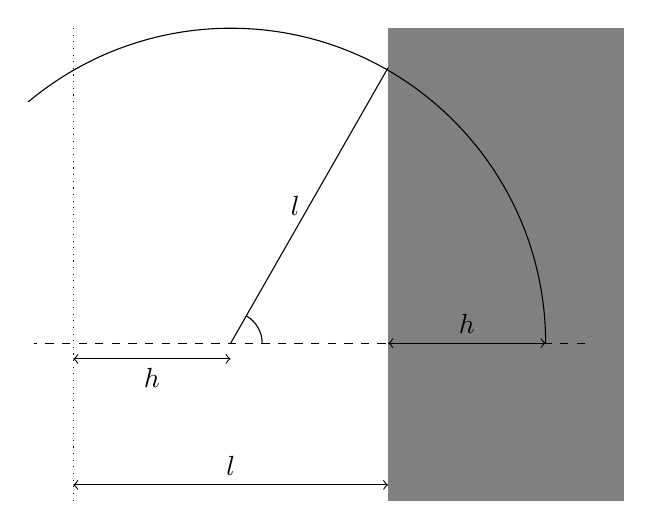
\begin{tikzpicture}

\fill[color=gray] (0,-2) rectangle (3,4);
\draw[style=dashed] (2.5,0) -- (-4.5,0);
\draw[style=dotted] (-4,-2) -- (-4,4);
\draw[<->] (-4,-1.8) -- node[above]{$l$} (0,-1.8);

\draw (2,0) arc (0:130:4cm);
\draw (-2,0) -- node[left]{$l$} (0,3.5);
\draw (-1.6,0) arc  (0:60:0.4cm);
\draw[<->] (0,0) --  node[above]{$h$} (2,0);

\draw[<->] (-4,-0.2) --  node[below]{$h$} (-2,-0.2);
\end{tikzpicture}

\vspace{1em}
Area of sphere is $4\pi l^{2}$.

Area of spherical cap inside the solid is $2\pi l h$.

\vspace{1em}
Fraction of spherical surface inside solid is:
\[ \phi(h) = \frac{2 \pi l h}{4 \pi l^{2}} = \frac{h}{2l}\]

Now, $h$ varies from 0 to $l$, as the atom position moves from the top of the layer into the wall.

So we know the fraction of atoms that hit the wall for a given distance $h$ inside the layer. To find the fraction for \emph{all} atoms in the layer, we \emph{average} over all positions in the layer. That is, we integrate over the layer, and divide by domain size:

\[ \phi = \frac{1}{l}\int_{0}^{l} \frac{h}{2l} \; dh = \frac{1}{2l^{2}} \int_{0}^{l} h \;dh = \frac{1}{2l^{2}} [\frac{1}{2} h^{2}]_{0}^{l} =
\frac{1}{4l^{2}}[l^{2} - 0] = \frac{1}{4}  \]

So, in time interval $t_{0}$, 1/4 of ensemble atoms within the layer hit the wall.

\vspace{1em}
Recall, the number of \emph{ensemble} atoms in layer is:
\[ \frac{\rho}{m} A l P(v_{ens}) \]

Thus, number hitting area $A$ per second is:
\[ \frac{\frac{1}{4} \frac{\rho}{m} A l P(v_{ens})  }{t_{0}} 
 = \frac{\rho A l P(v_{ens})}{ 4 m \frac{l}{v_{ens}}} =
 \frac{\rho A}{4 m} P(v_{ens}) v_{ens} \] 
Note that layer width $l$ has cancelled out.

\vspace{1em}
Define the `ensemble rain rate' as the number of particles with given speed $v_{ens}$ hitting the wall per second per unit area:
\[ R(v_{ens}) = \frac{\rho}{4 m} P(v_{ens}) v_{ens} \]

\vspace{1em}
To find the \emph{total} number of atoms hitting of \emph{all} speeds, we simply need to integrate over all speeds.  In other words, sum over all possible ensembles:

\[ R = \int_{0}^{\infty} R(v) \; dv = \int_{0}^{\infty} \frac{\rho}{4 m} P(v_{ens}) v_{ens} \; dv = \frac{\rho}{4 m} \int_{0}^{\infty} P(v_{ens}) v_{ens} \; dv \]

Now --- here's the cunning bit --- the construction $ \int P(v_{ens}) v_{ens} \; dv$ is just the \emph{average}. Hence:

\[ R = \frac{\rho \bar{v}}{4 m} \]

Note that we did \emph{not} need to know the specific statistical mechanical probability distribution for the particle speeds.


\subsubsection*{Lateral Momentum Transfer = Shear Stress}

Consider a bulk of water separated from a solid surface by a very thin gas layer of thickness $l$.  Assume $l$ is less than the mean free path in the gas, so that the previous analysis is valid.

Assume that the water bulk is moving, and that the bottom surface (facing the gas) has a constant tangential velocity $v_{s}$.

The gas is a vapour of liquid molecules, detaching and reattaching from the bulk liquid.  Each molecule detaches from the liquid in a random direction, with an \emph{average} tangential velocity of $v_{s}$.  Each atom has mass $m$, so has average lateral momentum $mv_{s}$. Each atom subsequently hits the solid surface, and sticks to the surface  --- an inelastic collision that transfers all of momentum $mv_{s}$ to the surface. 
% After some time, the gas molecule may separate from the surface, in a random %direction, with an \emph{average} tangential velocity of $0$.

\vspace{1em}
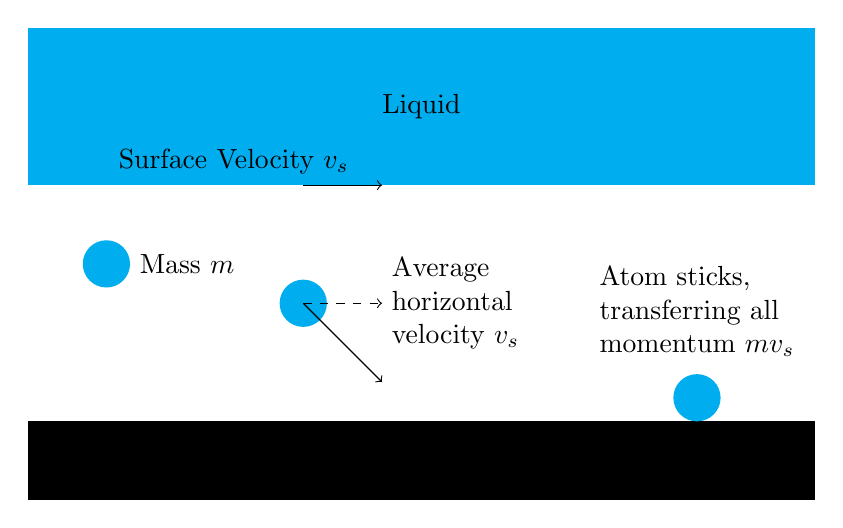
\begin{tikzpicture}

\fill[color=cyan] (0,3) rectangle (10,5);
\fill (0,0) rectangle (10,-1);

\node at (5,4) {Liquid};

\draw[->] (3.5,3) -- (4.5,3);
\node at (4.2,3.3) [left] {Surface Velocity $v_{s}$};

\fill[color=cyan] (1,2) circle (3mm);
\node at (1.3,2)[right] {Mass $m$};

\fill[color=cyan] (3.5,1.5) circle (3mm);
\draw[->] (3.5,1.5) -- (4.5,0.5);
\draw[->,dashed] (3.5,1.5) -- (4.5,1.5);
\node at (4.5,1.5) [right,align=left] {Average\\ horizontal\\ velocity $v_{s}$}; 

\fill[color=cyan] (8.5,0.3) circle (3mm);
\node at (8.5,0.7) [above,align=left] {Atom sticks,\\ transferring all\\ momentum $mv_{s}$};

\end{tikzpicture}

\vspace{1em}
Recall, the number of particles hitting the solid surface is $ \rho \bar{v} / 4 m$ per second per area.

Thus, momentum transferred to the surface per second per area:
\[ \frac{1}{A} \frac{dP}{dt} = \frac{\rho \bar{v}}{4 m} m v_{s} 
= \frac{1}{4} \rho \bar{v} v_{s}  \]

This force per unit area is a \emph{shear stress:}
\[ \sigma = \frac{1}{4} \rho \bar{v} v_{s} \]

Now, a velocity gradient in the bulk of a \emph{viscous} fluid of viscosity $\eta$ causes a shear stress:
\[ \sigma = \eta \left| \frac{dv(z)}{dz} \right| \]

At the surface, however, $dv/dz$ may be infinite, so surface shear stress may be better conceptualized --- by analogy with solid-solid friction --- with a friction coefficient $k$:
\[ \sigma = k v_{s} \]

Equating the gas kinetic shear stress with the frictive shear stress:
\[ \sigma = k v_{s} = \frac{1}{4} \rho \bar{v} v_{s} \]
\[ \Rightarrow k = \frac{1}{4} \rho \bar{v} \]

Alternatively, since $dv/dz$ is defined \emph{above} the surface, we may extrapolate $dv/dz$ down into the surface, getting the Navier slip condition:
\[ v_{s} = b \left| \frac{dv(z)}{dz} \right| \]

Equating frictive and viscous shear stresses, and substituting $v_{s}$:
\[\sigma = k v_{s} = k b \left| \frac{dv(z)}{dz} \right| = \eta \left| \frac{dv(z)}{dz} \right| \]

Therefore, quite generally:
\[ b = \frac{\eta}{k} \]


And for our de Gennes-inspired gas kinetic theory:
\[ b = \frac{4 \eta}{\rho \bar{v}} \]

This is the slip length in the Navier slip boundary condition as experienced by the fluid at the \textbf{bottom of the liquid.}  If we consider the slip length to be a parameter of the \textbf{solid} surface, then we must subtract the gas layer thickness $l$:
\[ b = -l + \frac{4 \eta}{\rho \bar{v}} \]
If the gas layer is only a few atom diameters thick, then $l < 1$ nm, thus is negligible.

de Gennes himself says: 
\[ b = -l + \frac{\eta}{\rho \bar{v}_{z}} \simeq  \frac{\eta}{\rho \bar{v}_{z}} \]

--- Note that I have corrected what I think are typos; his original paper says:
\[ b = -l + \frac{\eta}{\rho \bar{v}_{x}} \simeq  \frac{\eta}{\rho v_{z}} \]

\subsection*{Reconciling with de Gennes}

We use average speed (in any direction) $\bar{v}$. De Gennes used average speed \emph{in the z direction}, $\bar{v}_{z}$.

If \[ \bar{v} = 4 \bar{v}_{z} \] then our analyses are in perfect agreement.

De Gennes defines $\bar{v}_{z}$ like this:

\[ \bar{v}_{z} = \int_{0}^{\infty} \frac{1}{(2 \pi)^{1/2} v_{\mathrm{th}} }
v_{z} \mathrm{e}^{-v_{z}^{2} / 2v_{\mathrm{th}}^{2}}  \; \mathrm{d} v_{z} = v_{\mathrm{th}} / (2 \pi)^{1/2} \]

where $v_{\mathrm{th}}^{2} =  kT/m $.

That is:
\[ \bar{v}_{z} = \int_{0}^{\infty} \sqrt{\frac{m}{2 \pi k T}} v_{z} 
   \mathrm{e}^{\frac{- \frac{1}{2} m v_{z}^{2}}{kT}} \; dv_{z} = 
   \sqrt{\frac{kT}{2 \pi m}}\]
   
Now, in the Maxwell-Boltzmann statistics for an ideal gas, the distribution of a given \emph{component} of velocity is:
\[ f_{v}(v_{z}) = \sqrt{\frac{m}{2 \pi k T}} \exp
  \left[ \frac{-m v_{z}^{2}}{2 k T} \right] \]
  which is clearly what de Gennes is playing with.


This is a Gaussian distribution, therefore the average of $v_{z}$, given by
$ \int_{- \infty}^{\infty} f_{v}(v_{z}) v_{z} \; dv_{z}  $ is \textbf{zero.}

Hence, de Gennes's definition $\bar{v}_{z} = \int_{0}^{\infty} f_{v}(v_{z}) v_{z} \; dv_{z} $ is the average of the \textbf{absolute value} of $v_{z}$.

\vspace{1em}
So to reconcile.  The Maxwell-Boltzmann statistics yield an average value of the particle speed:
\[ \bar{v} = \sqrt{\frac{8 k T}{\pi m}} \]
which is:
\[ \bar{v} = \sqrt{\frac{8 k T}{\pi m}} = \sqrt{\frac{16 k T}{2 \pi m}}
   = \sqrt{16} \sqrt{\frac{k T}{2 \pi m}} = 4 \sqrt{\frac{k T}{2 \pi m}}
   = 4 \bar{v}_{z} \]
   
So we have found that $ \bar{v} = 4 \bar{v}_{z} $, hence our analysis and that of de Gennes reconcile perfectly.



\subsection*{Replicating de Gennes method}
The analysis of de Gennes used the $z$ component of velocity only, rather than the particle speed.
The following is an attempt to replicate de Gennes's analysis more directly, using $v_{z}$.

\vspace{1em}
Assume layer of thickness $l$, on some area $A$, giving a volume $Al$.

If gas has density $\rho$, and particle mass is $m$, then number of atoms in layer is: \[ \frac{\rho}{m} A l \]

\vspace{1em}
Split the gas into separate ensembles, each ensemble defined as the group of atoms all with the same $z$ velocity, $v_{z}$.  Then work with a single arbitrary ensemble.

An atom has probability $P(v_{z})$ of having ensemble velocity $v_{z}$.
Therefore, the ensemble indexed by $v_{z}$ contributes \[ \frac{\rho}{m} A l P(v_{z}) \] atoms to the layer.

\vspace{1em}
An atom at distance $l$ from the wall hits the wall in time $t_{0}$. An atom further away will not hit the wall in that time. Thus, the `isolation' time is:
\[ t_{0} = \frac {l} {v_{z}} \]

Considering only atoms from the same ensemble, only atoms that were in the layer to start with can possibly hit the wall in time $t_{0}$ --- hence the name `isolation' time.

%\vspace{1em}
%Considering ensemble atoms in the layer, in time $t_{0}$, what fraction of atoms hit the wall?

\vspace{1em}
%Answer: All of them. 
Since $t_{0}$ defines the time for the outermost particle to hit, and all the closer particles have the same $z$ velocity, then \emph{all} particles in the layer must hit in time $t_{0}$.

\vspace*{1em}
That is, all $ \frac{\rho}{m} A l P(v_{z}) $ ensemble atoms hit the wall in time $t_{0}$. So
\[ \frac{ \frac{\rho}{m} A l P(v_{z})  }{t_{0}} 
 = \frac{\rho A l P(v_{z})}{ m \frac{l}{v_{z}}} =
 \frac{\rho A}{m} P(v_{z}) v_{z} \] 
 
particles per second hit the wall.  Define the `ensemble rain rate' as particles hitting with given $z$ velocity per second \emph{per unit area:} 
\[ R(v_{z}) = \frac{\rho}{m} P(v_{z}) v_{z} \]

To find the \emph{total} number (per second per area) --- for any velocity --- we must integrate over $v_{z}$.

Equivalently, we must sum over all possible ensembles.  Each ensemble is indexed by its velocity $v_{z}$. The parameter $v_{z}$ ranges from $-\infty$ to $\infty$.
\[ \int_{-\infty}^{\infty} \frac{\rho}{m} P(v_{z}) v_{z} \;dv_{z} 
= \frac{\rho}{m} \int_{-\infty}^{\infty}  P(v_{z}) v_{z} \;dv_{z} \]

Now, the construction $\int P(z) v_{z} \; dv_{z}$ is the \emph{average}.

Problem: the $v_{z}$ parameter comes from the Gaussian distribution, which is \emph{symmetric}.  Therefore, the average is \emph{zero.}

The implicit assumption we have made is that all particles are heading \emph{towards} the wall i.e. $v_{z}>0$. In fact, at equilibrium, half of all atoms in the layer are heading \emph{away} from the wall.  Thus, only half of all particles in the layer contribute to the flux.

Resolution: Introduce a factor of $1/2$, and sum over all ensembles with positive $v_{z}$:
\[ R = \frac{1}{2}\int_{0}^{\infty} R(v_{z})\; dv_{z} = 
 \frac{1}{2} \frac{\rho}{m} \int_{0}^{\infty} P(v_{z}) v_{z} \;dv_{z} \]

This time, the construction $ \int_{0}^{\infty} P(v_{z}) v_{z} \;dv_{z} $ is equal to the average \textbf{absolute value} of $v_{z}$. If we denote this $\bar{v}_{z}$, then
\[ R = \frac{\rho \bar{v}_{z}}{2 m} \]

\subsubsection*{Momentum Transfer = Shear Stress}

Each particle leaving the liquid layer has an \emph{average} lateral velocity of $v_{s}$, the `slip' velocity of the bottom of the liquid. Each particle has mass $m$, so has lateral momentum $mv_{s}$.  Each particle hits the surface and sticks --- an inelastic collision that transfers all momentum to the surface.  Thus, each second, 
\[ \frac{\rho \bar{v}_{z}}{2 m} mv_{s} = \frac{1}{2} \rho \bar{v}_{z} v_{s} \]
kg ms$^{-1}$ of tangential momentum is transferred to a surface of unit area.

This is a shear stress:
\[ \sigma = \frac{1}{2} \rho \bar{v}_{z} v_{s} \]

In the bulk fluid, of viscosity $\eta$, a velocity gradient causes a shear stress:
\[ \sigma = \eta \frac{dv}{dz} \]

At the surface, however, $dv/dz$ may be infinite, so shear stress may be better conceptualized --- by analogy with solid-solid friction --- with a friction coefficient $k$:
\[ \sigma = k v_{s} \]

Or, since $dv/dz$ is defined above the surface, we may extrapolate $dv/dz$ into the surface, getting the Navier slip condition:
\[ v_{s} = b \frac{dv}{dz} \]

Substituting $v_{s}$, and equating frictive and viscous shear stresses:
\[ \sigma = k\; b \frac{dv}{dz} = \eta \frac{dv}{dz} \]

Therefore, quite generally: \[ b = \frac{\eta}{k} \]

\vspace{2em}
Here, we subsititute $v_{s}$ and equate gas kinetic and viscous shear stresses:
\[ \sigma = = \frac{1}{2} \rho \bar{v}_{z} v_{s} = 
\frac{1}{2} \rho \bar{v}_{z} b \frac{dv}{dz} = \eta \frac{dv}{dz} \]

Implying:
\[ b = \frac{2 \eta}{ \rho \bar{v}_{z}} \]

And as a bonus: 
\[ k = \frac{1}{2} \rho \bar{v}_{z} \]



\subsection*{Conclusion}
This expression for $b$ is a factor of 2 higher than de Gennes's formula.  Has he failed to account for half of the particles going away from the wall?  

\vspace{1em}
Crucially, it doesn't matter --- if slip lengths are twice as high as his prediction, this only strengthens the case for a thin gas layer causing slip.

Furthermore, we have derived an unambiguous expression using the particle \emph{speed}, which gives a still stronger case that a thin gas layer causes high slip.
\[ b = \frac{4 \eta}{\rho \bar{v}} \]


\end{document}